% !TEX root = ./Cours.tex
\documentclass[../€Cours-complet/Cours-complet]{subfiles}

\titleorchapter{Série de données}{10}
% Moyenne (moyenne pondérée) et représentations

\renewcommand{\arraystretch}{1.3}

\begin{document}

\maketitleCours

\section{Effectifs, fréquence, moyenne}

\begin{cours}[Effectif]
	Dans une série de données :
	\begin{itemize}
		\item L'\textbf{effectif} d'une donnée est le nombre de fois où cette donnée apparait.
		\item L'\textbf{effectif total} est la somme de tous les effectifs.
	\end{itemize}
\end{cours}

\begin{exemple}
	Voici les couleurs de cheveux des élèves dans une classe :

	\begin{center}
		\begin{tabular}{|c|c|c|c|}
			\hline
			Taille          & Blond & Brun & Noir
			\\ \hline
			Nombre d'élèves & $5$   & $12$ & $7$
			\\ \hline
		\end{tabular}
	\end{center}

	L'\textit{effectif} des élèves ayant les cheveux blonds est $5$.

	L'\textit{effectif total} est $5 + 12 + 7 = 24$.
\end{exemple}

\begin{cours}[Moyenne]
	Si les données sont des nombres, la \textbf{moyenne} de la série de données est égale à la somme de toutes ces données, divisées par l'effectif total.
\end{cours}

\begin{exemple}
	Si les cinq notes du semestre d'un élève sont $11$, $12$, $10$, $16$ et $18$, sa moyenne est

	$$ \dfrac{11 + 12 + 10 + 15 + 17}{5} = \dfrac{65}{5} = 13 $$
\end{exemple}

\begin{cours}[Fréquence]
	La \textbf{fréquence} d'une donnée est obtenue en divisant son effectif par l'effectif total :
	\begin{center}
		fréquence d'une donnée = $\dfrac{\text{effectif de la donnée}}{\text{effectif total}}$
	\end{center}
\end{cours}

\section{Diagrammes et graphiques}

\subsection{Diagramme en bâtons}

Dans un \textbf{diagramme en bâtons}, la hauteur d'un bâton est proportionnelle à l'effectif de la donnée associée.

\begin{exemple}
	Voici les notes d'un devoir de mathématiques:

	\begin{center}
		\begin{tabular}{|l|c|c|c|c|c|c|c|c|c|}
			\hline
			Note     & 2 & 3 & 4 & 5 & 6 & 7 & 8 & 9 & 10
			\\ \hline
			Effectif & 2 & 3 & 1 & 4 & 5 & 3 & 3 & 6 & 2
			\\ \hline
		\end{tabular}
	\end{center}

	À chaque note est associé un bâton : sa hauteur est le nombre d'élèves ayant obtenu cette note.

	\begin{center}
		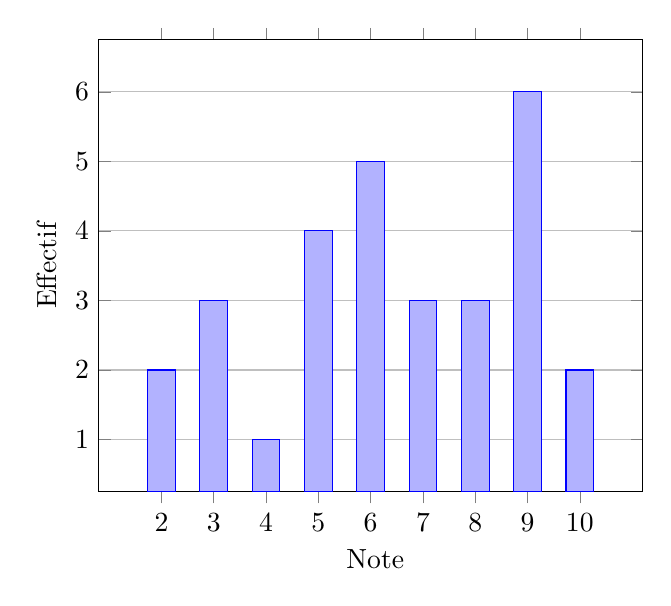
\begin{tikzpicture}
			\begin{axis}[
					width = 0.7\textwidth,
					ybar,
					enlargelimits=0.15,
					ylabel={Effectif},
					xlabel={\ Note},
					symbolic x coords={2, 3, 4, 5, 6, 7, 8, 9, 10},
					xtick=data,
					ymajorgrids = true,
					scaled y ticks = false,
					ytick=data,
				]
				\addplot coordinates { (2,2) (3,3) (4,1) (5,4) (6,5) (7,3) (8,3) (9,6) (10,2) };
			\end{axis}
		\end{tikzpicture}
	\end{center}
\end{exemple}

\subsection{Histogramme}

Lorsqu'il y a trop de données différentes, on peut les regrouper en \textbf{classes}, et utiliser un \textbf{histogramme}.

\begin{exemple}
	On a mesuré la taille des élèves dans le collège. Comme presque toutes ces tailles sont différentes, on les a regroupé en \textit{classes}, d'\textbf{amplitude} 5cm :


	\begin{center}
		\begin{tabular}{|l|c|c|c|c|c|c|}
			\hline
			Taille (en cm) & 135    & 140    & 145    & 150    & 155    & 160
			\\
			entre          & et 141 & et 146 & et 151 & et 156 & et 161 & et 166
			\\ \hline
			Effectif       & 75     & 161    & 255    & 182    & 117    & 143    % total : 913
			\\ \hline
		\end{tabular}
	\end{center}

	\begin{center}
		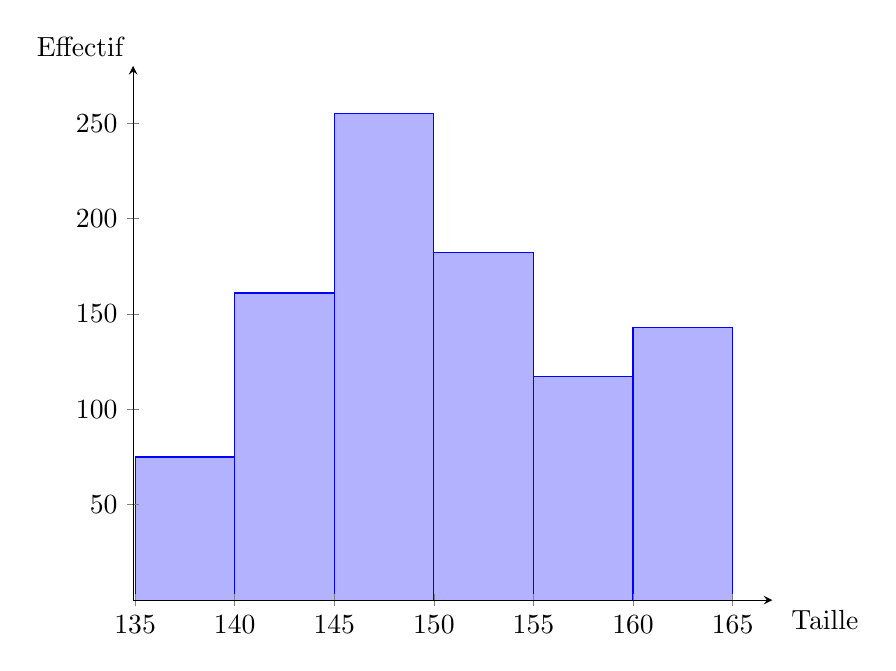
\begin{tikzpicture}
			\begin{axis}[
					width = 0.8\textwidth,
					xmin=134.9, xmax=167,
					ymin=0, ymax=280,
					axis lines=center,
					ylabel={Effectif},
					xlabel={\ Taille},
					xlabel style={below right},
					ylabel style={above left},
					area style,
				]
				\addplot+[ybar interval,mark=no] plot coordinates { (135,75) (140,161) (145,255) (150,182) (155,117) (160,143) (165,0) };
			\end{axis}
		\end{tikzpicture}
	\end{center}
\end{exemple}

\subsection{Diagramme circulaire}

Dans un \textbf{diagramme circulaire}, la mesure de chaque angle est proportionnelle à l'effectif associé.

\begin{exemple}
	Voici la répartition des élèves d'un collège en LV2 :

	\begin{center}
		\begin{tabular}{|l|c|c|c|c|c|}
			\hline
			Langue       & Allemand & Italien & Espagnol & Chinois & \textbf{Total}
			\\ \hline
			Effectif     & 40       & 40      & 70       & 30      & 180
			\\ \hline
			Angle (en °) & 80       & 80      & 140      & 60      & 360
			\\ \hline
		\end{tabular}
	\end{center}

	\begin{center}
		\begin{tikzpicture}
			\pie[
				text = inside,
				hide number,
				sum = auto
			]
			{
				40/Allemand,
				40/Italien,
				70/Espagnol,
				30/Chinois
			}
		\end{tikzpicture}
	\end{center}
\end{exemple}

\end{document}